\documentclass[12pt,a4paper,fleqn,titlepage]{report}
\usepackage[T1]{fontenc}
\usepackage{kpfonts,baskervald}
\usepackage[utf8]{inputenc}
\usepackage{listingsutf8}
\usepackage[italian]{babel}
\usepackage[italian]{varioref}
\usepackage{graphicx}
\usepackage[acronym]{glossaries}
\usepackage[style=numeric]{biblatex}
\usepackage{hyperref}
\usepackage{listings}
\usepackage{caption}

\lstset{
    basicstyle=\footnotesize\fontfamily{fvm}\selectfont,
    tabsize=2,
    keywordstyle=\color{black}\bfseries,
    numbers=left,
    columns=fullflexible,
    breaklines=true
}

\DeclareCaptionFormat{captionformat}{\textbf{#1} #2 #3}
\captionsetup[figure]{format=captionformat}
\captionsetup[table]{format=captionformat}

\hypersetup{
    colorlinks=true,
    linkcolor=black,
    urlcolor=black,
    citecolor=black
}

\addbibresource{references.bib}

\def\frontmatter{%
    \pagenumbering{Roman}
    \setcounter{page}{1}
    \renewcommand{\thesection}{\Roman{section}}
}%

\def\mainmatter{%
    \pagenumbering{arabic}
    \setcounter{page}{1}
    \setcounter{section}{0}
    \renewcommand{\thesection}{\arabic{section}}
}%

\def\backmatter{%
    \setcounter{section}{0}
    \renewcommand{\thesection}{\Alph{section}}
}%

\newcommand\blankpage{
    \clearpage
    \null
    \thispagestyle{empty}%
    %\addtocounter{page}{-1}%
    \clearpage
}

\newcommand\bd{\emph{\gls{big data}} }

% termini del glossario
\newglossaryentry{big data}{name={Big Data}, description={Insiemi di dati ad alta dimensionalità, spesso non strutturati, prodotti in maniera continuativa da un servizio o da dispositivi \glsentryshort{iot}}}
\newglossaryentry{mapreduce}{name={MapReduce}, description={Modello di programmazione per processare in maniera semplice operazioni, svolte su grandi dataset, eseguite su \gls{cluster} di grandi dimensioni}}
\newglossaryentry{bigtable}{name={Bigtable}, description={Sistema di archiviazione distribuito per dati strutturati}}
\newglossaryentry{cluster}{name={cluster}, description={Insieme di risorse computazionali}}
\newglossaryentry{fs}{name={file system}, description={Struttura dati utilizzata per la gestione dei dati archiviati su un supporto elettronico}}
\newglossaryentry{s3}{name={Amazon S3}, description={\Gls{fs} distribuito offerto da Amazon}}
\newglossaryentry{sched}{name={scheduler}, description={Strumento per la gestione di flussi di lavoro, nell'ambito specifico di questo elaborato, si intende per l'ingegnerizzazione di \gls{pipeline}}}
\newglossaryentry{pipeline}{name={data pipeline}, description={Sequenza di task che effettuano operazioni sui dati, in cui l'output di ogni task è usato come input dal successivo}}
\newglossaryentry{airflow}{name={Apache Airflow}, description={\Gls{sched} sviluppato da Airbnb e reso \textit{open source}}}
\newglossaryentry{luigi}{name={Luigi}, description={\Gls{sched} sviluppato da Spotify e reso \textit{open source}}}
\newglossaryentry{container}{name={Container}, description={Unità di virtualizzazione software che contiene un software unitamente alle sue dipendenze, senza virtualizzare un intero sistema operativo}}
\newglossaryentry{docker}{name={Docker}, description={Strumento per eseguire e amministrare i \gls{container}}}
\newglossaryentry{kube}{name={Kubernetes}, description={Orchestratore per gestire un \gls{cluster} composto da \gls{container}}}
\newglossaryentry{yarn}{name={Hadoop Yarn}, description={Yet Another Resource Negotiator, è la tecnologia di gestione delle risorse e pianificazione dell'esecuzione task nel framework di elaborazione distribuita open source Hadoop}}
\newglossaryentry{algoritmi all-reduce}{name={algoritmi all-reduce}, description={algoritmi utilizzati nell'ambito della computazione parallela, che aggregano gli \emph{array} (o i tensori) utilizzati da processi indipendenti in un'unica struttura dati}}

% acronimi
\newacronym{aws}{AWS}{Amazon Web Services}
\newacronym{cpu}{CPU}{Central Processing Unit}
\newacronym{dl}{DL}{Deep Learning}
\newacronym{emr}{EMR}{Elastic MapReduce}
\newacronym{gpu}{GPU}{Graphics Processing Unit}
\newacronym{ia}{IA}{Intelligenza Artificiale}
\newacronym{iot}{IoT}{Internet of Things}
\newacronym{mllib}{MLlib}{Machine Learning library}
\newacronym{ml}{ML}{Machine Learning}
\newacronym{ram}{RAM}{Random Access Memory}
\newacronym{sql}{SQL}{Structured Query Language}
\newacronym{api}{API}{Application Programming Interface}
\newacronym{dos}{DoS}{Denial of Service}
\newacronym{gmm}{GMM}{Gaussian Mixture Model}
\newacronym{knnc}{KNNC}{K-Nearest Neighbos Classifier}
\newacronym{lda}{LDA}{Linear Discriminant Analysis}
\newacronym{anova}{ANOVA}{ANalysis Of VAriance}
\newacronym{slr}{SLR}{Simple Linear Regression}
\newacronym{glr}{GLR}{Generalized Linear Regression}
\newacronym{glm}{GLM}{Generalized Linear Model}
\newacronym{pom}{POM}{Project Object Model}
\newacronym{xml}{XML}{eXtensible Markup Language}
\newacronym{musa}{MUSA}{Multilayered Urban Sustainability Action}
\newacronym{url}{URL}{Uniform Resource Locator}
\newacronym{eks}{EKS}{Elastic Kubernetes Service}
\newacronym{ec2}{EC2}{Elastic Compute Cloud}
\newacronym{iam}{IAM}{Identity and Access Management}
\newacronym{emrfs}{EMRFS}{EMR File System}
\newacronym{hdfs}{HDFS}{Hadoop Distributed File System}
\newacronym{rpc}{RPC}{Remote Procedure Call}
\newacronym{nccl}{NCCL}{NVIDIA Collective Communications Library}
\newacronym{tpu}{TPU}{Tensor Processing Unit}

\makeglossaries

\begin{document}

\frontmatter

\thispagestyle{empty}

\begin{center}
    
\includegraphics{images/logo.jpg}\\

    \vspace{.5cm}
    \textit{\textsf{Corso di Laurea in Sicurezza dei Sistemi e delle Reti Informatiche}} \\
    \vspace{1cm}
    {\huge Recupero e implementazione di componenti ML per analisi dati in un contesto distribuito} \\
    \vspace{2cm}
    \begin{flushleft}
        \textbf{Relatore} \\
        Prof. Claudio A. Ardagna \\
        \vspace{.7cm}
        \textbf{Correlatori} \\
        Prof. Marco Anisetti \\
        Dott. Antongiacomo Polimeno \\
        \vspace{1.5cm}
    \end{flushleft}
    \begin{flushright}
        \textit{Tesi di laurea di} \\
        \vspace{.25cm}
        Gabriele Stentella \\
        {\small 984491} \\
    \end{flushright}
    \vspace{.5cm}
    Anno Accademico 2023/2024 \\
\end{center}

\blankpage

\chapter*{Prefazione}
\pagestyle{plain}
Fra il 2003 e il 2006, Google divulgò tre componenti fondamentali sviluppati per affrontare la sfida di indicizzare internet: la tecnologia del proprio \gls{fs}, il modello \gls{mapreduce} e il sistema di archiviazione dati distribuito \gls{bigtable}; rivoluzionando l'industria nascente dei \gls{big data} e gettando le basi per lo sviluppo del framework \emph{Hadoop}, uno strumento \textit{open source} che ha consentito una larga adozione di tecniche per la computazione distribuita. Negli anni successivi, molte di quelle che ora sono le grandi aziende tecnologiche statunitensi hanno adottato e sviluppato l'ecosistema circostante \emph{Hadoop}, implementando diversi \gls{fs} distribuiti e framework per convertire le classiche interrogazioni \emph{\glsentryshort{sql}} in lavori \gls{mapreduce}. Dal momento che avviare e gestire un \gls{cluster} \emph{Hadoop} era un'operazione costosa e impegnativa, la vera adozione di massa dell'infrastruttura è avvenuta quando Amazon lanciò il suo servizio di cloud computing \textit{on-demand} e contestualmente \emph{\gls{emr}}, consentendo di sfruttare i vantaggi del modello \gls{mapreduce} impiegando il \gls{fs} distribuito \emph{\gls{s3}} senza dover acquistare e configurare l'hardware necessario.

Nel 2010 Google rilasciò una nuova ricerca in cui veniva illustrata un'architettura per \textit{query} distribuite e un formato di archiviazione utile a rendere efficienti le operazioni, ancora una volta ispirando altre aziende a sviluppare e poi rendere \textit{open source} tecnologie come \emph{Apache Impala}, \emph{Presto} e \emph{Apache Parquet}.

Alcuni anni dopo vennero rilasciate le prime versioni di \emph{Apache Spark} che ottennero da subito un grande successo, infatti era molto semplice migrare da sistemi per interrogazioni \emph{\glsentryshort{sql}} di \emph{Hadoop} a \emph{SparkSQL}, e il nuovo framework aveva una sintassi più semplice e migliori performance di \gls{mapreduce}, grazie alla sua capacità di utilizzare la \glsentryshort{ram} come cache. La gestione delle risorse del cluster era gestita attraverso il \textit{resource manager} \emph{\gls{yarn}}.
Poco dopo \emph{Spark} cominciò ad avere successo anche nel mondo del \gls{ml}, grazie al framework \emph{Apache Mahout} prima, e poi alla \emph{\gls{mllib}}, più veloce; inoltre le possibilità offerte da \emph{Spark} si ampliarono grazie alla nascita di \gls{sched} come \emph{\gls{airflow}} e \emph{\gls{luigi}}.

Fra il 2013 e il 2014 si diffusero \emph{\gls{docker}} e l'orchestratore \emph{\gls{kube}} che semplificarono la gestione di cluster anche di grandi dimensioni, rendendo le architetture molto spiù stabili e scalabili; \emph{Spark} si è adattato al contesto, permettendo di utilizzare proprio \emph{\gls{kube}} come \textit{resource manager}.

Con l'avvento del \gls{dl} le attività di computazione si sono spostate sull'utilizzo massiccio di \glsentryshort{gpu} e sull'impiego delle più importanti librerie di \emph{Python} dedicate, \emph{Tensorflow} e \emph{Pytorch}, dunque per questi carichi di lavoro si è passati all'utilizzo delle \gls{api} proprietarie delle librerie per distribuire la computazione anziché usare \emph{Spark}, in modo da usare in maniera efficente la \glsentryshort{gpu} ed evitare di dover creare un cluster per poi installare le librerie su tutti i componenti.

Il percorso che si intende illustrare in questo elaborato ha previsto sia una fase di recupero di algoritmi \gls{ml} eseguiti in un ambiente distribuito attraverso \emph{Spark}, sia l'implementazione di nuovi elementi che sfruttano le \gls{api} delle moderne librerie \gls{dl}, nell'introduzione viene analizzato lo scenario di partenza che rappresenta il contesto in cui si inserisce il lavoro di tesi, in modo tale da illustrare nel dettaglio le motivazioni alla base dell'attività svolta, per poi descrivere il contributo dato dalla soluzione proposta e dettagliare la struttura della trattazione che segue.

\blankpage

\tableofcontents
\listoffigures

\blankpage

\mainmatter

\chapter*{Introduzione}
La presenza sempre più diffusa dei \bd ha reso necessario avere infrastrutture e tecnologie di analisi adatte ad estrarre valore da tali dati e che siano scalabili per essere utilizzate da realtà di diverse dimensioni. Al fine di avere procedure efficaci sia nell'attività di analisi che in quella di costruzione di modelli predittivi, occorre affrontare i problemi tipici dei \bd che sono la diffusa eterogeneità, l'accumulo di rumore in fase di raccolta, la frequente presenza di correlazioni spurie. Gli algoritmi impiegati devono essere anche accurati dal punto di vista statistico ed efficaci per quanto riguarda il carico computazionale; per tutte queste ragioni, ma in modo particolare per la necessità di efficenza computazionale, i \bd hanno portato allo sviluppo di nuove infrastrutture di computazione e nuovi metodi di memorizzazione dei dati \cite{fan:2014}.

In tale contesto, le tecnologie di \emph{Apache Hadoop} prima e \emph{Apache Spark} poi, hanno reso semplice ed economica l'analisi e la memorizzazione dei dataset di grandi dimensioni, in particolare, dal momento che l'analisi di \bd richiede una sperimentazione reiterata per trovare i parametri corretti e individuare le giuste metriche di valutazione, \emph{Spark} rappresenta una soluzione tecnologicamente adatta a supportare in modo efficiente questo tipo di lavoro, in particolare se viene utilizzata la libreria \gls{mllib} per il \textit{design} e il \textit{tuning} di algoritmi \gls{ml} \cite{salloum:2016}.

Negli ultimi anni, oltre agli algoritmi \gls{ml} di \textit{shallow learning}, hanno avuto molto successo i modelli \gls{dl} che, a differenza delle architetture \textit{shallow}, traggono vantaggio dall'avere un grande numero di parametri liberi, quindi l'addestramento di tali modelli vede nei \bd una risorsa fondamentale, e contemporaneamente necessita di metodi efficenti per la parallelizzazione delle operazioni di \textit{training} \cite{xue-wenchen:2014}.

I benefici dati da un'analisi dati svolta con l'ausilio di algoritmi \gls{ml} o modelli \gls{dl} sono evidenti nel campo della ricerca medica e scientifica, nella gestione di infrastrutture critiche e nella cosiddetta \emph{business intelligence} \cite{bharadiya:2023}, ma la letteratura è sempre più ricca di applicazioni di queste tecnologie nel campo della sicurezza informatica: grazie alla presenza pervasiva dell'\gls{iot} e in generale dell'evoluzione tecnologica dei dispositivi informatici, compresi gli strumenti di rete, c'è una grandissima produzione di dati che possono essere analizzati in tempo reale per eseguire azioni di prevenzione, ricerca di minacce e \textit{incident response}. Soltanto alcune fra le numerose applicazioni in questo campo sono l'analisi del traffico di rete con l'obiettivo di istituire uno schema di priorità e rendere meno efficaci eventuali attacchi \gls{dos}, identificare comportamenti sospetti, individuare malware e integrare i sistemi di autenticazione \cite{sarker:2023}. In particolare, l'uso dei classificatori è utile per implementare dei filtri sia sul traffico web sia sulla corrispondenza di posta elettronica, in modo tale da ridurre la probabilità che il personale di un'azienda entri in contatto con contenuti malevoli, e di conseguenza minimizzare l'impatto di email spam o siti web malevoli sulla rete aziendale o di un'infrastruttura critica; i classificatori in questione devono essere allenati con un insieme di dati molto grande e in continuo aggiornamento, in modo tale che stiano al passo con l'evoluzione delle minacce, inoltre è necessario che, in base al tipo di classificazione, venga utilizzato un modello statistico adeguato.

L'obiettivo del lavoro svolto durante il tirocinio interno, è quello di recuperare degli algoritmi \gls{ml} di analisi dati che sono stati sviluppati in linguaggio Java e utilizzano la tecnologia \emph{Spark}, con il fine di renderli eseguibili in un ambiente distribuito, superando il \textit{resource manager} originario \gls{yarn} e utilizzando \gls{kube}. Parallelamente al recupero degli algoritmi esistenti, la tesi si pone l'obiettivo di studiare la tecnologia di esecuzione distribuita della libreria \emph{Tensorflow} per lo sviluppo di nuovi algoritmi per l'analisi dati eseguibili nel medesimo ambiente distribuito dei precedenti. L'infrastruttura finale — pensata per lo storage sicuro e l'elaborazione di \bd — in cui si sono eseguiti gli algoritmi, è un ambiente distribuito amministrato con l'orchestratore \gls{kube} ed è stata implementata nell'ambito del progetto \gls{musa} finanziato dal Ministero dell’Università e della Ricerca attraverso il Piano Nazionale di Ripresa e Resilienza.

L'elaborato è organizzato come segue: nel primo capitolo si espone lo stato dell'arte delle tecnologie per l'analisi dati e il calcolo distribuito, in modo tale da introdurre gli aspetti tecnici alla base del lavoro svolto; nel secondo capitolo si illustrano gli algoritmi coinvolti nella tesi; nel terzo capitolo viene descritto nel dettaglio il lavoro svolto, seguendo la divisione del lavoro nelle fasi di \textit{development}, \textit{deployment} e \textit{testing}; nel quarto e ultimo capitolo si riassume il contributo dato da questa tesi e si esplorano i possibili sviluppi futuri.

\chapter{Le tecnologie per l'analisi dati e il calcolo distribuito}
    \section{L'\glsentryshort{ia} per l'analisi dati}\label{sec:ai}

    \section{Apache Spark}

    \section{Docker}

    \section{Kubernetes}\label{sec:kubernetes}


\chapter{Gli algoritmi di analisi dati}
Una parte fondamentale del lavoro svolto è stata quella di recuperare degli algoritmi \gls{ml} e statistici sviluppati in linguaggio Java, sfruttando le librerie offerte da Spark, di seguito si descrivono in dettaglio le tecniche di inferenza e gli algoritmi implementati dai task.
    \paragraph{K-means clustering}
    K-means è un algoritmo di clustering con approccio partizionale, ottiene in input il parametro $k$, numero di cluster, poi la computazione inizia selezionando $k$ centroidi casuali dal dataset su cui è eseguito, viene calcolata la distanza fra ogni punto del dataset e i centroidi, in modo da assegnare ogni dato al cluster relativo al centroide più vicino. Ogni volta che un nuovo punto viene assegnato al cluster, il centro viene ricalcolato, quindi l'algoritmo viene eseguito iterativamente finché i cluster non sono stabili (nessun punto viene più assegnato a un nuovo cluster) \cite{ikotun:2023}.
    Osservando il clustering come un \emph{learning problem} — ovvero trattandolo come un compito di apprendimento automatico in cui l'obiettivo è assegnare automaticamente gli oggetti in gruppi omogenei — si utilizza l'algoritmo K-means per allenare un modello \gls{ml} che possa essere sfruttato per poi svolgere delle predizioni: fornito un nuovo punto che rappresenta un dato non presente nel dataset con cui si è svolto il \emph{training}, il modello deve essere in grado di collocarlo in uno dei cluster che ha individuato. Fra i task implementati, uno è dedicato alla creazione del modello e uno all'utilizzo di tale modello per svolgere le predizioni; è inoltre presente un task dedicato alla valutazione del modello, sfruttando il \emph{Silhouette score} \cite{shahapure:2020}.
    Nella versione classica dell'algoritmo la metrica utilizzata è la distanza euclidea, ma sono state proposte diverse alternative al fine di migliorare le performance \cite{chen:2021, chen:2021a, shen:2017}.
    La variante bisecting K-means \cite{steinbach:2000} sfrutta l'algoritmo di base per implementare una procedura differente: inizialmente il dataset è considerato come un unico cluster e viene utilizzato K-means per dividerlo in due cluster, si ripete il processo un certo numero di volte e poi si tiene la sezione che presenta due cluster con la più alta similarità fra gli elementi, infine vengono iterati i passaggi precedenti fino a raggiungere il numero di cluster desiderato. Come nel caso dell'algoritmo di base, anche bisecting K-means viene utilizzato per creare un modello con cui poi effettuare delle predizioni.

    \paragraph{Decision Tree Classifier}
    I classificatori ad albero sono modelli predittivi con una struttura assimilabile a un diagramma di flusso, ideali per il data mining supervisionato. Ogni nodo dell'albero è un test su un attributo del dato da classificare, ogni ramo è un possibile esito del test e ogni foglia indica l'etichetta di classificazione. Il nodo radice non ha rami in ingresso ed è infatti il punto di ingresso all'albero stesso. La classificazione viene effettuata eseguendo i test rappresentati dai nodi, di volta in volta scegliendo il test successivo sulla base del risultato del precedente, continuando fino all'ultimo livello (terminale), in cui tutte le tuple di dati in un nodo comprendono campioni di una sola classe.
    La costruzione del modello avviene seguendo la fase di generazione (\textit{generation}) prima e di potatura (\textit{pruning}) poi; nella prima fase tutte i dati di allenamento partono nel nodo radice, viene definito un criterio di divisione ed è selezionato il miglior attributo per effettuare la divisione, dopodiché i dati vengono partizionati nei nodi figli e la procedura è ripetuta fino a quando aggiungendo nodi foglia non si aumenta più la precisione dei nodi foglia. Nella seconda fase si punta a ridurre le dimensioni del modello in modo da renderlo più efficente, in particolare vengono rimossi i sottoalberi che si sono creati per riflettere le caratteristiche di eventuale rumore nei dati o outliers \cite{priyanka:2020}.
    Una volta che si ha un modello affidabile ed efficente, lo si può utilizzare per la classificazione di dati.

    \paragraph{Gaussian Mixture Model}
    Si tratta di un modello statistico utilizzato per rappresentare la distribuzione di probabilità di un insieme di dati come una combinazione di più distribuzioni gaussiane. Un \gls{gmm} assume che i dati siano generati da un insieme di sottopopolazioni, ognuna che segue una distribuzione gaussiana. È definito da un numero specifico di componenti gaussiane, ognuna con la propria media e varianza; l'obiettivo dell'algoritmo è quello di costruire un modello sulla base di un certo insieme di dati, in modo tale da eseguire poi predizioni collocando nuovi dati nella gaussiana corretta (ovvero stimando la variabile latente) \cite{reynolds:2015}.
    Il modello viene costruito utilizzando la classe offerta da Spark GaussianMixtureModel in un task, poi un secondo utilizza il modello per eseguire le predizioni.

    \paragraph{K-Nearest Neighbors Classifier}
    L'algoritmo k-nearest neighbors \cite{cover:1967} è stato utilizzato per costruire un classificatore, quindi il task che lo implementa ha l'obiettivo di restituire in output la classe a cui appartiene un oggetto che riceve in input. La classificazione avviene scegliendo la classe più comune fra i $k$ oggetti con features più simili (e quindi "vicini") all'oggetto da classificare, dove $k$ è parametro dell'algoritmo.
    Dal momento che il funzionamento dell'algoritmo si basa sul confronto della distanza fra l'oggetto da classificare e una serie di oggetti conosciuti, la fase di allenamento del modello consiste nell'estrazione delle caratteristiche dai dati dedicati al training, in modo da rappresentare ogni oggetto come un vettore in uno spazio $n$-dimensionale (dove $n$ è il numero delle caratteristiche). Ogni vettore è in seguito assegnato a una classe sulla base della classificazione indicata nel dataset, si tratta dunque di un metodo di apprendimento supervisionato e non parametrico \cite{siegel:1957}: non vengono fatte assunzioni sulla distribuzione dei dati su cui opera l'algoritmo, rendendolo adatto alla classificazione di dati di cui non si conosce la distribuzione; occorre tenere presente, tuttavia, che il meccanismo con cui avviene la classificazione, comprende intrinsecamente il rischio che la classificazione sia svolta con bassa accuratezza nel caso in cui la distribuzione sia fortemente asimmetrica, perché gli esempi di una classe più frequente tendono a dominare la previsione di un nuovo esempio (tendono ad essere comuni tra i $k$ vicini più prossimi a causa del loro grande numero), per questo sono stati proposte delle alternative alla regola di base del voto a maggioranza dei $k$ vicini \cite{coomans:1982}.
    Utilizzando le classi di Spark dedicate al modello \glsentryshort{knnc} — KNNClassificationModel e KNNClassifier — viene costruito il classificatore sulla base di un dataset in input, per poi utilizzare il modello per effettuare le predizioni.

    \paragraph{Linear Discriminant Analysis}
    Si tratta un algoritmo di riduzione della dimensionalità e di classificazione utilizzato nell'ambito dell'apprendimento supervisionato. L'obiettivo è trovare la combinazione lineare delle caratteristiche che massimizza la separazione tra le classi dei dati utilizzati nell'allenamento del modello, per farlo l'algoritmo \glsentryshort{lda} proietta i dati in uno spazio delle caratteristiche a dimensioni inferiori, senza perdere informazioni, in modo che le diverse classi siano il più separabili possibile lungo questa nuova dimensione. Vengono calcolate le medie delle caratteristiche per ciascuna classe, oltre alle matrici di dispersione intra-classe (\emph{data spread} all'interno di una classe) e inter-classe (\emph{data spread} fra le classi). Successivamente si calcolano le direzioni discriminanti, ovvero i vettori che massimizzano il rapporto tra la varianza inter-classe e la varianza intra-classe, i dati vengono proiettati su queste direzioni per ridurre la dimensionalità e separare le classi nel nuovo spazio delle caratteristiche.
    Dopo la proiezione dei dati, è possibile utilizzare un classificatore per classificare i nuovi dati in base alla loro posizione nello spazio delle caratteristiche ridotto.
    \glsentryshort{lda} è spesso utilizzato come tecnica di riduzione della dimensionalità prima di applicare un classificatore, poiché aiuta a migliorare le prestazioni del modello riducendo il rischio di overfitting. È da notare che vengono fatte le assunzioni che i dati siano distribuiti normalmente e che le classi abbiano matrici simili \cite{tharwat:2017}.
    Nel task implementato, vengono utilizzate le classi di clustering offerte da Spark LDA e LDAModel per allenare il modello ed effettuare le predizioni.

    \paragraph{Principal Component Analysis}
    In modo simile a \glsentryshort{lda}, questo algoritmo mira a ridurre la dimensionalità dei dati ed è quindi utilizzato nel \emph{preprocessing}; l'idea di base è quella di estrarre le informazioni importanti dal dataset, per poi rappresentarle come variabili ortogonali (le componenti principali) ottenute come combinazioni lineari delle variabili originali, in modo tale da poter poi distinguere graficamente i diversi cluster.
    Per estrarre la prima componente si ricerca quella che ha varianza maggiore, perché in questo modo si estrae la maggior quantità di informazione dal dataset, per la seconda si pone il vincolo di ortogonalità con la prima e si cerca nuovamente quella con varianza maggiore (tolta la prima), reiterando il processo un numero pari alle componenti che si desidera estrarre \cite{abdi:2010}.
    Più nel dettaglio, il processo consiste in una prima normalizzazione dei dati (sottraendo la media e dividendo per la deviazione standard), per poi calcolare la matrice di covarianza ($\sigma$) dei dati, in seguito si calcolano autovalori e autovettori di $\sigma$, vengono selezionate le componenti principali estraendo gli autovettori con i corrispondenti autovalori più grandi, infine si proiettano i dati normalizzati sulle componenti principali estratte per ridurre la dimensionalità.
    Grazie alle classi di Spark PCA e PCAModel, il task esegue il \emph{fitting} del modello e poi restituisce un dataset con le informazioni relative alle componenti principali.

    \paragraph{\gls{anova}}
    \gls{anova} è una tecnica di inferenza statistica utilizzata per analizzare la differenza fra le medie di più gruppi differenti di dati, con il fine di descrivere le relazioni presenti fra le variabili presenti nel dataset. È particolarmente utile per analizzare i dati ottenuti da diverse misurazioni svolte in seguito a diversi generici "trattamenti" eseguiti nel corso di un esperimento, perché consente di valutare la significanza statistica dei "trattamenti" confrontando i dati con quelli di un ipotetico gruppo di controllo. Per utilizzare \gls{anova} si assume che ogni gruppo su cui si sono effettuate le misurazioni segua una distribuzione normale, le varianze delle popolazioni di provenienza dei gruppi siano uguali fra loro, le osservazioni sui vari gruppi siano indipendenti; l'ipotesi nulla è che tutte le medie delle diverse popolazioni considerate siano uguali, quindi che non ci sia una differenza significativa fra i diversi gruppi, mentre l'ipotesi alternativa è che almeno una media sia differente, con un certo livello di significanza.
    La versione più semplice dell'analisi è \emph{one-way \gls{anova}}, in cui viene esaminata l'influenza di una singola variabile indipendente, ed è quella eseguita dal task nel caso in cui il dataset in input sia composto da sole due colonne (una per la variabile dipendente e una per quella indipendente); la versione \emph{two-way \gls{anova}}, che analizza l'influenza di due differenti variabili indipendenti, è eseguita se il dataset ha tre colonne, la versione \emph{multi-way \gls{anova}} serve per l'analisi della varianza provocata da più di due variabili indipendenti simultaneamente ed è eseguita se il dataset ha almeno quattro colonne.
    L'algoritmo restituisce una tabella contenente i gradi di libertà, la somma dei quadrati, la media dei quadrati, l'\emph{f-ratio}, il \emph{p-value}, il numero di celle del dataset, la somma e la media dei loro valori. L'\emph{f-ratio} è il rapporto fra la varianza tra i diversi gruppi, e la varianza all'interno dei singoli gruppi, mentre il \emph{p-value} è la probabilità che l'\emph{f-ratio} sia maggiore o uguale del valore atteso, calcolato prendendo direttamente il valore della \emph{F-distribution} per il valore di significanza $\alpha$, considerando i gradi di libertà di numeratore e denominatore dell'\emph{f-ratio}; se \emph{p-value} è minore di $\alpha$ l'ipotesi nulla è falsa, quindi c'è una differenza significativa dal punto di vista statistico fra le medie dei gruppi \cite{scheffe:1999}.

    \paragraph{Linear Regression}
    La regressione lineare è una tecnica statistica utilizzata per modellare la relazione tra una variabile dipendente e una o più variabili indipendenti, in modo da definire la variabile dipendente come una combinazione lineare di alcuni valori (le variabili indipendenti), detti predittori perché una volta individuata la relazione fra tali valori e la variabile dipendente, è possibile effettuare delle predizioni sulla base dei valori osservati. La forma più comune è la regressione lineare semplice (\gls{slr}), che coinvolge una sola variabile indipendente, ma esistono diverse varianti della regressione lineare che possono essere utilizzate in diverse situazioni.
    L'obiettivo di \gls{slr} è quello di trovare una funzione lineare che predica il valore della variabile dipendente dato un certo valore di quella indipendente (ovvero data l'ascissa, il valore dell'ordinata deve essere una predizione accurata): le predizioni sono svolte sulla base di un solo predittore \cite{seber:2012}.

    Un \gls{glm} è una generalizzazione che mira a rendere più flessibile la regressione lineare classica, in cui le variabili coinvolte possono seguire una distribuzione arbitraria, e viene utilizzata una \emph{link function} che mette in relazione i predittori con la media della distribuzione della variabile dipendente; anziché far variare linearmente la variabile dipendente stessa, in questo modello è una funzione di tale variabile che varia linearmente con i predittori. La regressione lineare è un \gls{glm} in cui la distribuzione della variabile dipendente è una normale con varianza costante e la \emph{link function} è l'identità \cite{dobson:2018}.
    Il task implementato offre la possibilità di scegliere, con un opportuno parametro, se utilizzare la \gls{slr} o la \gls{glr} che utilizza un \gls{glm}.

    \paragraph{Logistic Regression}
    Nel caso in cui si abbia a che fare con delle variabili che possono assumere soltanto due valori (circostanza frequente nei classificatori), è possibile utilizzare un particolare tipo di regressione — la regressione logistica — che utilizza la funzione logit per associare ad un vettore in ingresso un valore di probabilità di appartenenza ad una delle due classi possibili \cite{dobson:2018, hosmer:2013}.
    Per costruire un modello \gls{ml}, durante la fase di addestramento (supervisionato) si utilizzano i dati dedicati per trovare i coefficienti della funzione logit che massimizzano la corrispondenza fra i dati e la loro classe di appartenenza, poi viene stabilito il \emph{decision boundary} per separare le diverse classi nello spazio delle features. Una volta allenato il modello, si può utilizzare per effettuare classificazione presentando in ingresso nuovi dati: l'output del modello è la probabilità che il vattore in ingresso rappresenti un oggetto appartenente a una delle due classi. I task implementati offrono anche la possibilità di vedere i parametri necessari alla valutazione del modello (precision, recall, f-score) e l'evoluzione della precisione del modello durante la fase di addestramento.

    % \paragraph{Naive Bayes}

    % \paragraph{Random Forest Tree}

    % \paragraph{Linear Support Vector Classifier}

\chapter{Recupero e implementazione degli algoritmi}
\section{Operazioni preliminari}
La prima fase del lavoro è consistita nel recupero di alcuni algoritmi sviluppati con tecnologia Spark sfruttando la libreria \gls{mllib}, originariamente implementati nell'ambito del progetto EVOTION \cite{anisetti:2018}. Affinché i singoli Spark task fossero eseguibili singolarmente, dopo una prima analisi del codice già sviluppato, si è resa necessaria l'estrazione delle singole classi Java che implementano i diversi algoritmi e la contestuale creazione di un progetto autonomo per ogni algoritmo.
L'autonomia dei singoli progetti è un requisito necessario per avere la possibilità di creare in maniera semplice i cosiddetti \emph{fat jar} (o \emph{uber jar}) — maggiori dettagli in seguito — e dal momento che le classi sono state estratte da un progetto più grande, è stato necessario risolvere le dipendenze perché ogni algoritmo potesse importare tutte le classi e librerie esterne di cui necessitava.
Un'ulteriore attività svolta è stata quella di aggiornamento della versione di Spark dalla 2.2.0 alla 3.5.0, mantenendo Java 8; dal momento che numerosi algoritmi fra quelli coinvolti nel lavoro utilizzano la classe "VectorDisassembler", realizzata in Scala 2.11 per Spark 2.2.0 da un singolo sviluppatore e non più aggiornata, è stata creata una \emph{fork} della classe in modo da poter aggiornare la versione di Scala e così rendere il codice compatibile con Spark 3.5.0.

\paragraph{Maven}
I progetti Java sono stati gestiti con Apache Maven, uno strumento per l'amministrazione di progetti software, quindi per risolvere le dipendenze e aggiornare la versione di Spark, l'attività svolta è stata quella di scrivere un nuovo file \gls{pom} per ogni algoritmo; tale file è in formato \gls{xml} e comprende sia i dettagli di configurazione del progetto, sia le informazioni necessarie a Maven per realizzare il pacchetto contenente l'applicazione Java. Il file \gls{pom} contiene delle sezioni che sono dedicate alla struttura del progetto, ovvero in cui sono indicate le relazioni fra le diverse classi; una sezione dedicata alle proprietà del progetto (strettamente dipendenti dal linguaggio e dalle tecnologie utilizzate); una sezione dedicata alla fase di costruzione del pacchetto dell'applicazione Java, dove possono essere configurati vari plugin; un'ultima sezione in cui sono indicate tutte le dipendenze del progetto.
All'interno di un singolo progetto possono esserci diversi file \gls{pom}, ognuno che gestisce una parte del codice, a diversi livelli di dettaglio: un file più generale può indicare soltanto l'identificativo del gruppo (package) di cui fa parte il progetto, l'identificativo dell'artifatto e i diversi moduli che lo compongono; i file dei singoli moduli poi possono specificare i plugin necessari alla costruzione del file \emph{jar}, così come le dipendenze. Alcuni algoritmi prevedono la presenza di un task Spark dedicato soltanto all'allenamento del modello e un task diverso per effettuare predizioni utilizzando il modello allenato; in questo caso è stato organizzato un unico progetto in cui i due task sono moduli di uno stesso artefatto generale. Un esempio di file \gls{pom} generale è riportato nell'appendice \ref{apx:general_pom}, mentre un esempio di un file di un singolo modulo, contenente sia i plugin sia le dipendenze, è riportato nell'appendice \ref{apx:module_pom}.
Il funzionamento di Maven si basa sull'utilizzo dei plugin, ovvero degli strumenti che combinano più azioni in sequenza per rendere semplice la compilazione, il testing, il deployment e altre attività comuni durante lo sviluppo software. I plugin vengono configurati all'interno del file \gls{pom}, nell'ambito del lavoro di questa tesi, sono stati configurati, per ciascun task, Apache Maven Assembly Plugin \cite{assembly:2024} e Log4j Transform Maven Plugin \cite{logging:2023}. Il primo consente di costruire un archivio che contiene anche le dipendenze, i moduli, la documentazione, mentre il secondo serve per ottimizzare le chiamate di logging alle API di Log4j, infatti inserisce le chiamate di logging in posizioni statiche, in modo tale da non dover calcolare a runtime la posizione.

\paragraph{\emph{Uber jar}}
Gli applicativi Java sono solitamente "confezionati" in file archivio, chiamati JAR (da Java Archive), che comprendono sia i file di diverse classi Java, sia i relativi metadati e tutte le risorse che utilizzano; queste generiche risorse possono essere sia file di testo o multimediali, sia altri file JAR.
I file JAR sono un aspetto fondamentale del linguaggio Java, sia per quanto riguarda la facilità di distribuzione sia per la sicurezza, infatti è possibile inserire in un unico file, detto \emph{uber jar} o \emph{fat jar}, tutti i file delle classi sviluppate per l'applicativo, uniti a tutte le classi che costituiscono le dipendenze, rendendo l'archivio un file completamente autonomo, ovvero eseguibile senza necessità di importare nessuna classe esterna.

\paragraph{Aggiornamento della versione di Spark}
In particolare, l'attività di aggiornamento e riorganizzazione del codice si è svolta in più fasi in cui sono state prima risolte le dipendenze delle classi relative ai singoli algoritmi, svolgendo un test con un dataset di esempio per ciascun task, lanciando l'esecuzione direttamente dall'interno dell'ambiente di sviluppo, in seguito è stata aggiornata la versione di Spark, e sono state svolte minime modifiche al codice Java delle classi per risolvere alcuni problemi di compatibilità relativi all'aggiornamento, solitamente dovuti al fatto che nella nuova versione di Spark alcune classi sono state spostate in librerie differenti rispetto alla versione 2.2.0. Per l'aggiornamento della classe "VectorDisassembler", dopo aver effettuato la \emph{fork} del codice, si è aggiornato il file \gls{pom}, poi si è costruito il nuovo file \emph{jar} che è stato in seguito importato da tutti i task che lo richiedevano.

Il plugin Maven Assembly è stato configurato in modo tale che venisse incluso il \emph{Classpath} (\lstinline{<addClasspath>true</addClasspath>}), è stata specificata la classe principale da eseguire una volta avviato l'archivio finale (\lstinline{<mainClass>it.unimi.evotion.tasks.kmeans_model.KmeansModel</mainClass>}), è stato inserito il tipo di descrittore da utilizzare per nominare l'assembly JAR (\lstinline{<descriptorRef>jar-with-dependencies</descriptorRef>}) e poi si è specificata la fase del ciclo di vita di Maven in cui eseguire l'istanza di esecuzione (\lstinline{<phase>package</phase>}). Una volta aggiornati i file di configurazione di tutti i progetti relativi ai singoli algoritmi, sono stati costruiti i file \emph{uber jar}.

\section{Esecuzione su un cluster Kubernetes locale}
Al fine di rendere eseguibili i task Spark in un ambiente distribuito gestito con \gls{kube}, è stato fatto un primo test di esecuzione in container \gls{docker} dei singoli \emph{fat jar}, in modo tale da individuare un'immagine di partenza che soddisfasse le necessità delle singole classi, inoltre, a puro scopo dimostrativo si è anche effettuata una prova di esecuzione su un cluster \gls{kube} eseguito su una sola macchina. In questa fase, sia il file archivio del task sia il dataset di lavoro sono stati aggiunti all'immagine \gls{docker} utilizzata per la costruzione dei pod \gls{kube}, tuttavia nella configurazione finale, come verrà illustrato in seguito, il file eseguibile e i dati non sono inseriti nell'immagine, ma vengono letti da un sistema di storage distribuito. Per ottenere un'immagine \gls{docker} da usare in \gls{kube}, è stato usato lo strumento \lstinline{docker-image-tool.sh}, messo a disposizione dalla distribuzione Spark, utile per costruire e pubblicare immagini \gls{docker} in maniera immediata.

Il \gls{cluster} locale è stato configurato su un dispositivo Apple MacBook Pro con processore Apple M1 Pro e 16 GB di memoria unificata, impostando l'applicativo \gls{docker} desktop (utilizzato anche per la gestione del \gls{cluster} \gls{kube}) in modo tale che potesse usare fino a 8 core di CPU e 13 GB di memoria. Da \gls{docker} desktop è stato attivato \gls{kube}, in modo tale che venisse configurato un \gls{cluster} con un singolo nodo (master) che contiene i pod dedicati a: \gls{api} server, controller manager, scheduler, etcd, coredns, kube-proxy (si faccia riferimento alla sezione \ref{sec:kubernetes} per la spiegazione delle funzioni dei singoli pod).
Una volta configurato il \gls{cluster}, si è utilizzato lo script \lstinline{spark-submit} per avviare l'esecuzione dei task sul \gls{cluster}; con questa procedura viene impartito il comando all'\gls{api} server che si occupa di creare un nuovo pod che funge da Spark driver, a sua volta, il driver crea gli esecutori e si connette a tali nodi, per poi eseguire il codice dell'applicazione.

\begin{figure}
    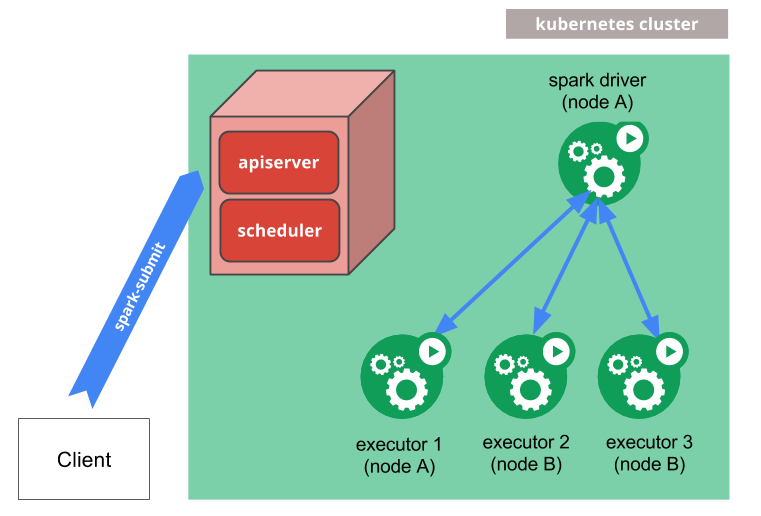
\includegraphics[width=\linewidth]{images/spark-on-kube.png}
    \caption[Funzionamento di \lstinline{spark-submit}]{Funzionamento di \lstinline{spark-submit}\\ \footnotesize{\textit{Fonte:} \url{https://spark.apache.org/docs/3.5.0/running-on-kubernetes.html}}}
\end{figure}

Per rendere più agevole l'attività di recupero degli algoritmi, si è scelto di configurare le proprietà di Spark non attraverso le \gls{api} di Java, ma con i parametri dello strumento \lstinline{spark-submit}, in questo modo non è stato necessario modificare il codice e in più se ne favorisce il riuso, perché al variare dell'infrastruttura di deployment non serve apportare modifiche al codice, ma basta cambiare i paramentri dello strumento di lancio. Di seguito si riportano le impostazioni utilizzate per il lancio sul \gls{cluster} locale:
\begin{enumerate}
    \item \lstinline{--master} serve per indicare l'\gls{url} dello Spark master, in particolare l'indirizzo dell'\gls{api} server \gls{kube};
    \item \lstinline{--deploy-mode} definisce dove istanziare il nodo driver, in modalità \lstinline{client} è avviato localmente e quindi si interfaccia ai nodi del \gls{cluster} come nodo esterno, mentre in modalità \lstinline{cluster} viene avviato direttamente sui nodi worker;
    \item con \lstinline{--class} si specifica la classe da eseguire all'interno dell'archivio JAR;
    \item il termine indicato in \lstinline{--name} è quello utilizzato da \gls{kube} per nominare le risorse create per l'esecuzione dei task, come i driver e gli executors;
    \item attraverso l'utilizzo di \lstinline{--conf} si possono impostare diverse proprietà per la configurazione di Spark, in particolare è utile indicare il namespace in cui avviare i pod per eseguire il task (con \lstinline{spark.kubernetes.namespace}) e l'immagine con cui avviare i container (con \lstinline{spark.kubernetes.container.image}), inoltre nel caso in cui sia necessaria l'autenticazione per avere il permesso di esecuzione all'interno del \gls{cluster}, si indica l'account con \lstinline{spark.kubernetes.authenticate.driver.serviceAccountName}.
\end{enumerate}
Oltre ai parametri di configurazione, lo strumento richiede che venga indicato il JAR dell'applicazione da eseguire ed eventuali argomenti, nel caso dei task Spark coinvolti nel lavoro, è stato indicato il percorso interno all'immagine in cui è stato inserito l'archivio Java, il percorso del dataset e gli argomenti specifici per ciascun algoritmo.

\section{Esecuzione su un cluster AWS EKS}
Per avvicinarsi alla configurazione di deployment finale, si è configurato un \gls{cluster} \gls{kube} utilizzando il servizio di cloud computing \gls{eks} offerto da \gls{aws}. Sfruttando lo strumento \lstinline{eksctl} si è creato un \gls{cluster} di istanze di tipo \gls{ec2} \emph{m5.xlarge} — indicate per computazione "general batch processing" — dotate di 4 CPU virtuali e 16 GiB di memoria, ed è stato esposto l'accesso remoto tramite ssh. All'interno del \gls{cluster} si è creato un namespace dedicato all'esecuzione dei task, poi una mappatura (\emph{iamidentitymapping}) fra uno specifico utente \gls{kube} e il ruolo dedicato all'amministrazione dei container, in seguito è stato creato un ruolo \gls{iam} per l'esecuzione dei task e vi è stata associata una policy che consentisse l'accesso completo ad uno specifico bucket \gls{s3} e al servizio di monitoraggio Amazon CloudWatch, così come una policy per consentire l'amministrazione dei \gls{cluster} virtuali e il lancio di "job" software (fare riferimento all'appendice \ref{apx:policy} per il contenuto delle policy citate). Infine è stato creato un \gls{cluster} virtuale per l'esecuzione vera e propria dei task, indicando come provider dei container il \gls{cluster} fisico appena configurato.

Con un'infrastruttura così configurata, è possibile sia eseguire i task utilizzando direttamente lo strumento \lstinline{spark-submit}, come precedentemente illustrato, ma eseguendolo da un nodo appartenente al cluster, oppure si può utilizzare \gls{eks} StartJobRun, uno strumento pensato appositamente per l'esecuzione di Spark task in un cluster \gls{eks}, attraverso il quale viene configurato indirettamente \lstinline{spark-submit}. Nell'appendice \ref{apx:startjob} si può vedere l'esempio di configurazione dello strumento per l'esecuzione del task che implementa l'algoritmo kmeans: con questa nuova configurazione, a differenza dell'esecuzione su cluster locale, l'archivio JAR e il dataset passati al tool di esecuzione, così come il percorso in cui scrivere i risultati dell'algoritmo, non sono locali all'immagine eseguita dal container nel \gls{cluster}, ma sono percorsi in un bucket \gls{s3}; la comunicazione fra lo Spark driver e il bucket S3 avviente attraverso \gls{emrfs}, un'implementazione di \gls{hdfs} usata per leggere e scrivere file dai cluster \gls{emr} a \gls{s3} \cite{emrfs:2024}.

\begin{figure}
    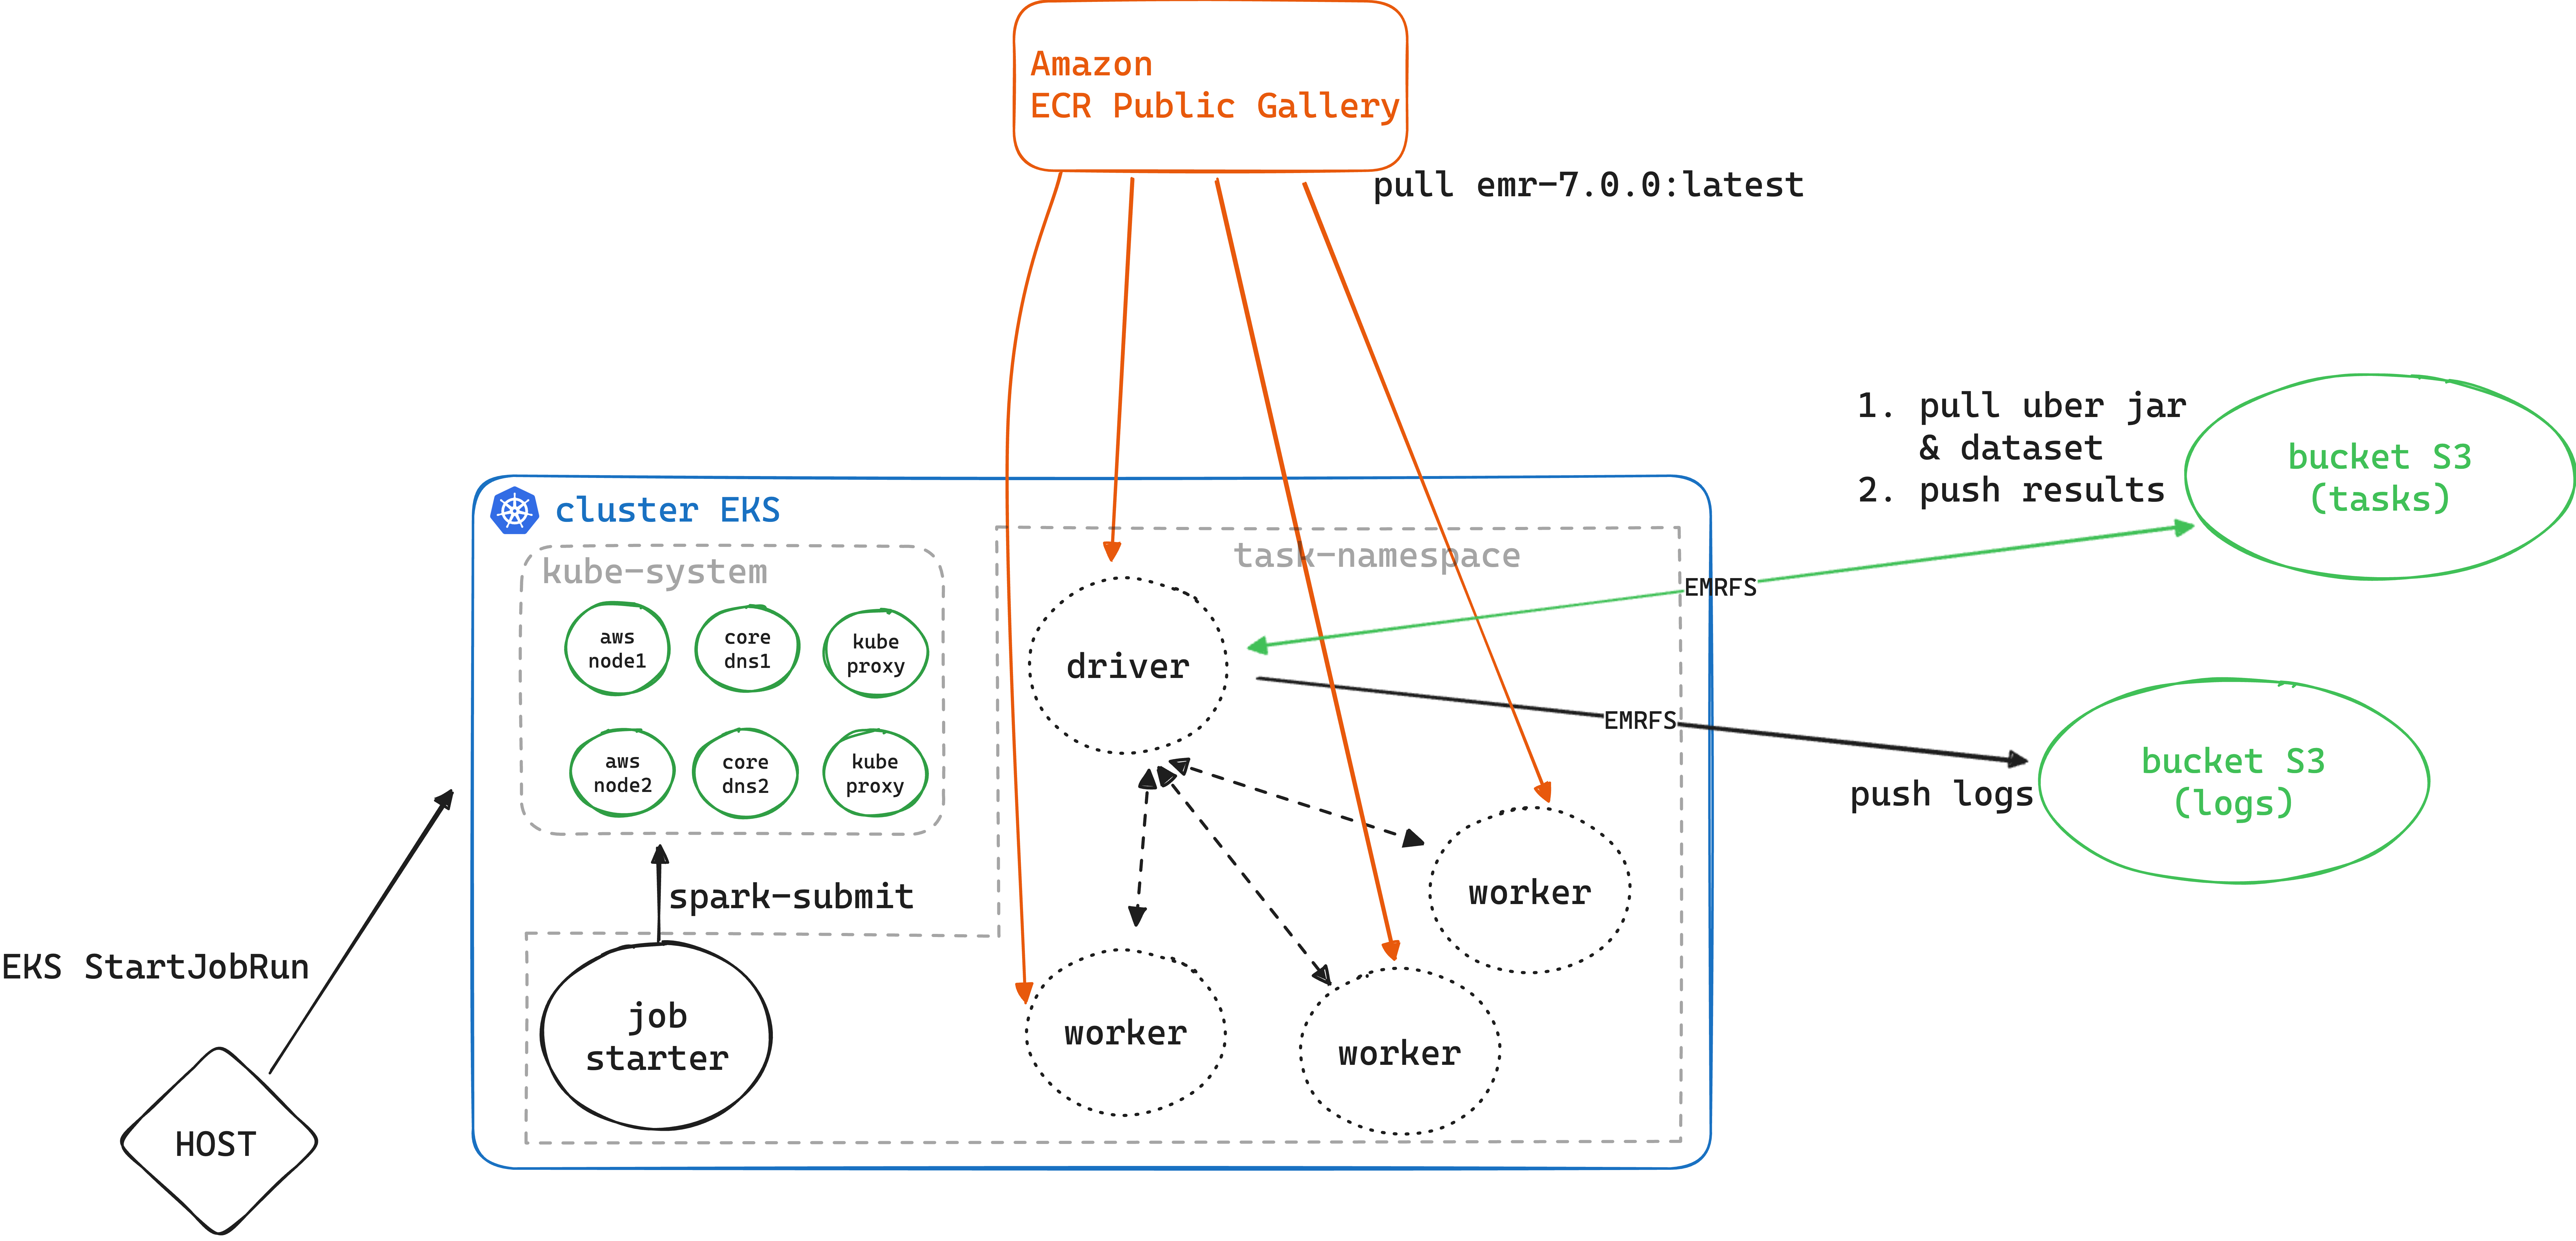
\includegraphics[width=\linewidth]{images/infrastructure.png}
    \caption{Schema riassuntivo dell'infrastruttura configurata con Amazon EKS}
\end{figure}

\section{Test di performance dell’esecuzione distribuita}
Per dimostrare l'effettiva distribuzione del carico computazionale sul \gls{cluster} si sono svolte molteplici esecuzioni degli algoritmi \gls{ml} sia sull'infrastruttura \gls{kube} locale, sia su quella sul servizio di cloud computing, misurando il tempo di esecuzione ed analizzando sia i file di log sia le informazioni riguardanti lo stato del \gls{cluster} nel corso dell'esecuzione dei task.

Il flusso di lavoro generale atteso e che si è osservato è il seguente:
\begin{itemize}
    \item Il nodo dedicato allo Spark master richiede a \gls{kube} un numero di esecutori (executors) pari a quello indicato nella fase di lancio del workload, quindi viene creato un numero di pod pari al numero di executors;
    \item Gli indirizzi IP di ciascun executor sono registrati nel \gls{cluster} e gli viene assegnato un numero identificativo;
    \item Lo Spark master assegna l'esecuzione di un task a ogni executor, fino a quando non sono finiti tutti i task set di tutti i passi che compongono il workload;
    \item Una volta che tutti i task sono stati completati e i nodi executors hanno riportato il risultato allo Spark driver, il lavoro è concluso, quindi gli executors vengono terminati e il pod dedicato allo Spark driver entra nello stato "completed" (qualora il workload preveda la scrittura dei risultati in specifici file, tale azione viene fatta dal driver).
\end{itemize}

Dall'analisi dei file di log — di cui si riporta un estratto per quanto riguarda l'esecuzione di un algoritmo sul cluster \gls{aws} \gls{eks} nell'appendice \ref{apx:logs} — si è trovata conferma della corretta esecuzione.

\section{Studio e implementazione di un algoritmo di test in Tensorflow}
Come illustrato nella sezione \ref{sec:ai}, la libreria Tensorflow è estremamente utilizzata in molti ambiti del machine learning, grazie alla sua semplicità d'uso e alla possibilità di ottimizzare l'esecuzione su hardware specifico, pertanto si è studiata l'implementazione di nuovi algoritmi sfruttando la libreria in questione, superando l'approccio con Java, pur mantenendo la possibilità di esecuzione su \gls{cluster} Spark.

Tensorflow ha la sua \gls{api} — \lstinline{tf.distribute} — che permette la distribuzione sia della computazione da parte di modelli predittivi già allenati, sia del training; è pensata per funzionare sia con il codice che utilizza \gls{api} fornite da librerie di alto livello, come \lstinline{Model.fit} di Keras, sia con programmi che usano Tensorflow più a basso livello, come quelli con \emph{training step} personalizzati \cite{tfdis:2024}.
La grande automazione presente nei componenti della libreria Tensorflow consente di distribuire la computazione del codice applicando delle modifiche minime: occorre definire una "strategia" di distribuzione, utilizzare metodi specifici per configurare i dispositivi coinvolti in modo da comunicargli il ruolo che devono assumere nella computazione, creare il modello all'interno dello \emph{scope} della strategia appena definita. Di seguito si discute nel dettaglio ciascun passaggio.

\paragraph{Definizione della strategia}
Le strategie si differenziano sia per la tipologia di piattaforma hardware che utilizzano, sia per la modalità di parallelizzazione del training che sfruttano, quest'ultima può essere sincrona, quindi con tutti i \emph{workers} che lavorano contemporaneamente su diverse sezioni del dataset di input e poi effettuano una sincronizzazione ad ogni step, oppure asincrona, ovvero con un lavoro indipendente e aggiornamento asincrono delle variabili.
Esistono 7 differenti strategie di distribuzione del calcolo:
\begin{enumerate}
    \item per distribuire il training in maniera sincrona su più \gls{gpu} su uno stesso dispositivo, viene utilizzata MirroredStrategy, con cui viene creata una replica per ogni variabile del modello su ciascuna \gls{gpu}, poi i valori sono tenuti sincronizzati e vengono aggiornati utilizzando efficenti \gls{algoritmi all-reduce} che solitamente usano \gls{nccl};
    \item TPUStrategy viene usata per effettuare il training distribuito su un \gls{cluster} di Tensor Processing Units;
    \item la strategia adottata in questo lavoro, MultiWorkerMirroredStrategy, serve per la distribuzione sincrona su diversi dispositivi, offrendo la possibilità di avere più \gls{gpu} su ciascun dispositivo, crea una copia di ogni variabile del modello su ciascun worker. La comunicazione fra i dispositivi può avvenire con \gls{rpc} (compatibile CPU e \gls{gpu}) o \gls{nccl} (solo per \gls{gpu});
    \item con ParameterServerStrategy si implementa un \gls{cluster} per il training asincrono, composto da parameter server e da worker, dove i primi creano e conservano le variabili del modello, mentre i secondi leggono le variabili dai server per poi aggiornarle e riscriverle sui server, senza mai sincronizzarsi fra loro;
    \item un'altra strategia utilizzabile su un solo dispositivo è CentralStorageStrategy, la quale prevede che le variabili siano soltanto sulla CPU, mentre le operazioni di aggiornamento sono svolte distribuite sulle \gls{gpu};
    \item OneDeviceStrategy serve per memorizzare tutte le variabili ed eseguire qualsiasi funzione su uno specifico dispositivo, come una singola \gls{gpu};
    \item la strategia di default, ovvero quella utilizzata nel caso in cui non venga definita una delle altre strategie, non distribuisce il carico computazionale, serve soltanto per scrivere librerie o programmi che possano gestire ogni tipo di distribuzione e funzionino anche senza distribuire la computazione.
\end{enumerate}

\paragraph{Configurazione}
Una volta definita la strategia, qualora si voglia parallelizzare la computazione su un \gls{cluster}, bisogna configurare i dispositivi coinvolti in modo tale che conoscano il ruolo che devono assumere nel training o nell'utilizzo del modello predittivo. Nel caso di TPUStrategy si utilizzano direttamente le \gls{api} Tensorflow per indicare l'indirizzo del \gls{tpu} cluster resolver, connettersi e inizializzare il sistema, poi la distribuzione è gestita in maniera automatica dalla libreria.
Con strategie che coinvolgono realmente più worker, come MultiWorkerMirroredStrategy e ParameterServerStrategy, si ha un controllo preciso su tutti i dispositivi del \gls{cluster}: nella variabile d'ambiente TF\_CONFIG, scritta con formato JSON, si configura la sezione \lstinline{cluster} — un dizionario contenente gli indirizzi IP e i numeri di porta di tutti i nodi del cluster, distinguendo fra \lstinline{worker} ed eventualmente parameter server (\lstinline{ps}) (è un'informazione uguale per tutti i nodi) — e la sezione \lstinline{task} che specifica il tipo e l'indice di un nodo specifico, quello con indice pari a 0 per prassi è il nodo chief che, oltre a svolgere i compiti di un normale worker, si occupa anche di salvare i checkpoint e scrivere i \emph{summary files} per TensorBoard. In aggiunta alla configurazione dei singoli nodi, è possibile definire la modalità di comunicazione fra dispositivi, utilizzando le \gls{api} di Tensorflow e scegliendo fra \gls{rpc} (\lstinline{CommunicationImplementation.RING}) e \gls{nccl} (\lstinline{CommunicationImplementation.NCCL}).

L'unica modifica al codice necessaria per distribuire il training, una volta definita la strategia, è quella di effettuare le chiamate alle \gls{api} per costruire e compilare il modello all'interno dello scope della strategia.

\paragraph{Deployment su \gls{cluster} \gls{kube}}
Per fare training distribuito con TensorFlow è preferibile configurare il cluster con uno StatefulSet anziché un Deployment in modo tale che ogni pod abbia un'identità stabile in rete; così facendo, ogni replica dello StatefulSet rappresenta un nodo worker.
Per eseguire un task in maniera distribuita, è stato creato un file in formato yaml, in cui è stato configurato uno StatefulSet con 3 repliche, su ognuna delle quali è stata definita la variabile TF\_CONFIG in modo tale che ciascuna replica conoscesse gli indirizzi degli altri componenti del \gls{cluster}. Il codice python del modello — una rete neurale convoluzionale per il riconoscimento dei caratteri scritti a mano — è stato inserito in un'immagine \gls{docker}, caricata su Docker Hub, in questo modo al momento della creazione del \gls{cluster} si è fatto il pull dell'immagine, poi è stato eseguito il codice su ciascun pod.

\paragraph{Deployment su un \gls{cluster} Spark esistente}
Qualora si voglia distribuire il training su un cluster Spark già esistente, all'interno dell'ecosistema Tensorflow è stato sviluppato un apposito componente che consente la distribuzione in maniera immediata. La funzione \lstinline{MirroredStrategyRunner} all'interno del pacchetto \lstinline{spark_tensorflow_distributor} può essere utilizzata in un modo del tutto simile a quello descritto nei precedenti paragrafi, infatti è costruita sulla base di MultiWorkerMirroredStrategy. L'utilizzo classico prevede di incapsulare il codice da eseguire su un singolo nodo all'interno di una funzione, poi si passa tale funzione a \lstinline{MirroredStrategyRunner.run()}, eventualmente configurando il runner in modo tale da definire i seguenti parametri: il numero totale di \gls{gpu} o CPU utilizzabili da Spark (\lstinline{num_slots}), se deve essere eseguito in locale sullo Spark driver o distribuito sui worker (\lstinline{local_mode}), se deve utilizzare la \gls{gpu} (\lstinline{use_gpu}), il nome della risorsa che Spark usa per lo scheduling della \gls{gpu} (\lstinline{gpu_name}), se il codice fornito per il singolo worker implementa una strategia personalizzata — ovvero una di quelle elencate precedentemente — o meno (\lstinline{use_custom_strategy}).

\section{Deployment su infrastruttura MUSA}

\chapter{Conclusioni}


\appendix
\chapter{\glsentryshort{pom} generale}\label{apx:general_pom}
\begin{lstlisting}
<project xmlns="http://maven.apache.org/POM/4.0.0" xmlns:xsi="http://www.w3.org/2001/XMLSchema-instance"
         xsi:schemaLocation="http://maven.apache.org/POM/4.0.0 https://maven.apache.org/xsd/maven-4.0.0.xsd">
    <modelVersion>4.0.0</modelVersion>

    <groupId>it.unimi.evotion.tasks</groupId>
    <artifactId>kmeans-task</artifactId>
    <version>1.0</version>
    <packaging>pom</packaging>

    <modules>
        <module>kmeans</module>
        <module>kmeans_model</module>
        <module>kmeans_predict</module>
    </modules>
</project>
\end{lstlisting}

\chapter{\glsentryshort{pom} di un singolo modulo}\label{apx:module_pom}
\begin{lstlisting}
<?xml version="1.0" encoding="UTF-8"?>
<project xmlns="http://maven.apache.org/POM/4.0.0"
         xmlns:xsi="http://www.w3.org/2001/XMLSchema-instance"
         xsi:schemaLocation="http://maven.apache.org/POM/4.0.0 http://maven.apache.org/xsd/maven-4.0.0.xsd">
    <modelVersion>4.0.0</modelVersion>

    <parent>
        <groupId>it.unimi.evotion.tasks</groupId>
        <artifactId>kmeans-task</artifactId>
        <version>1.0</version>
    </parent>

    <artifactId>kmeans</artifactId>
    <name>KMeans</name>
    <version>1.0</version>

    <properties>
        <maven.compiler.source>1.8</maven.compiler.source>
        <maven.compiler.target>1.8</maven.compiler.target>
        <project.build.sourceEncoding>UTF-8</project.build.sourceEncoding>

        <spark.version>3.5.0</spark.version>
        <scala.version>2.12</scala.version>
    </properties>

    <build>
        <plugins>
            <plugin>
                <artifactId>maven-assembly-plugin</artifactId>
                <configuration>
                    <archive>
                        <manifest>
                            <addClasspath>true</addClasspath>
                            <mainClass>it.unimi.evotion.tasks.kmeans.Kmeans</mainClass>
                        </manifest>
                    </archive>
                    <descriptorRefs>
                        <descriptorRef>jar-with-dependencies</descriptorRef>
                    </descriptorRefs>
                </configuration>
                <executions>
                    <execution>
                        <id>make-assembly</id>
                        <phase>package</phase>
                        <goals>
                            <goal>single</goal>
                        </goals>
                    </execution>
                </executions>
            </plugin>
            <plugin>
                <groupId>org.apache.logging.log4j</groupId>
                <artifactId>log4j-transform-maven-plugin</artifactId>
                <version>0.1.0</version>
                <executions>
                    <execution>
                        <goals>
                            <goal>process-classes</goal>
                        </goals>
                    </execution>
                </executions>
            </plugin>
        </plugins>
    </build>

    <dependencies>
        <dependency>
            <groupId>org.apache.spark</groupId>
            <artifactId>spark-core_${scala.version}</artifactId>
            <version>${spark.version}</version>
            <scope>provided</scope>
        </dependency>
        <dependency>
            <groupId>org.apache.spark</groupId>
            <artifactId>spark-sql_${scala.version}</artifactId>
            <version>${spark.version}</version>
            <scope>provided</scope>
        </dependency>
        <dependency>
            <groupId>org.apache.spark</groupId>
            <artifactId>spark-mllib_${scala.version}</artifactId>
            <version>${spark.version}</version>
            <scope>provided</scope>
        </dependency>
        <dependency>
            <groupId>org.apache.spark</groupId>
            <artifactId>spark-streaming_${scala.version}</artifactId>
            <version>${spark.version}</version>
            <scope>provided</scope>
        </dependency>
        <dependency>
            <groupId>org.apache.logging.log4j</groupId>
            <artifactId>log4j-api</artifactId>
            <version>2.22.1</version>
        </dependency>
        <dependency>
            <groupId>org.apache.logging.log4j</groupId>
            <artifactId>log4j-core</artifactId>
            <version>2.22.1</version>
        </dependency>
        <dependency>
            <groupId>org.apache.spark.ml.feature</groupId>
            <artifactId>VectorDisassembler</artifactId>
            <version>1.0</version>
        </dependency>
    </dependencies>
</project>
\end{lstlisting}

\chapter{\gls{iam} policies}\label{apx:policy}
Trust policy per la creazione del ruolo per l'esecuzione dei task, si consente al solo utente \emph{admin} di assumere il ruolo:
\begin{lstlisting}
{
  "Version": "2012-10-17",
  "Statement": [
    {
      "Effect": "Allow",
      "Principal": { "AWS": "arn:aws:iam::[ID]:user/admin" },
      "Action": "sts:AssumeRole"
    }
  ]
}
\end{lstlisting}
\textit{Nota: rispetto al file originale, l'ID del cluster è stato sostituito da \emph{\lstinline{[ID]}}.}

Policy che garantisce l'accesso al bucket \gls{s3} di logging (situato all'Amazon Resource Name indicato) e a CloudWatch, associata al ruolo sopracitato:
\begin{lstlisting}
{
    "Version": "2012-10-17",
    "Statement": [
        {
            "Effect": "Allow",
            "Action": [
                "s3:PutObject",
                "s3:GetObject",
                "s3:ListBucket"
            ],
            "Resource": [
                "arn:aws:s3:::logs-tasks-stentella",
                "arn:aws:s3:::logs-tasks-stentella/*"
            ]
        },
        {
            "Effect": "Allow",
            "Action": [
                "logs:CreateLogStream",
                "logs:DescribeLogGroups",
                "logs:DescribeLogStreams"
            ],
            "Resource": [
                "arn:aws:logs:*:*:*"
            ]
        },
        {
            "Effect": "Allow",
            "Action": [
                "logs:PutLogEvents"
            ],
            "Resource": [
                "arn:aws:logs:*:*:log-group:task-group:log-stream:task/*"
            ]
        }
    ]
}
\end{lstlisting}

Policy per l'amministrazione dei cluster virtuali e il lancio dei Job:
\begin{lstlisting}
{
    "Version": "2012-10-17",
    "Statement": [
        {
            "Effect": "Allow",
            "Action": [
                "iam:CreateServiceLinkedRole"
            ],
            "Resource": "*",
            "Condition": {
                "StringLike": {
                    "iam:AWSServiceName": "emr-containers.amazonaws.com"
                }
            }
        },
        {
            "Effect": "Allow",
            "Action": [
                "emr-containers:CreateVirtualCluster",
                "emr-containers:ListVirtualClusters",
                "emr-containers:DescribeVirtualCluster",
                "emr-containers:DeleteVirtualCluster"
            ],
            "Resource": "*"
        },
        {
            "Effect": "Allow",
            "Action": [
                "emr-containers:StartJobRun",
                "emr-containers:ListJobRuns",
                "emr-containers:DescribeJobRun",
                "emr-containers:CancelJobRun"
            ],
            "Resource": "*"
        }
    ]
}
\end{lstlisting}

\chapter{Configurazione di EKS StartJobRun}\label{apx:startjob}
\begin{lstlisting}
{
    "name": "kmeans",
    "virtualClusterId": "[VIRTUAL-ID]",
    "executionRoleArn": "arn:aws:iam::[ID]:role/EMRContainers-JobExecutionRole",
    "releaseLabel": "emr-7.0.0-latest",
    "jobDriver": {
        "sparkSubmitJobDriver": {
            "entryPoint": "arn:aws:s3:::test-tasks-stentella/kmeans-1.0-jar-with-dependencies.jar",
            "entryPointArguments": ["s3://test-tasks-stentella/dataset.csv", "5",
            "s3://test-tasks-stentella/result"],
            "sparkSubmitParameters": "\
            --master k8s://https://E5F648AFE82BAF20017B44F112918FBE.gr7.us-east-1 \
            .eks.amazonaws.com \
            --class it.unimi.evotion.tasks.kmeans.Kmeans \
            --conf spark.kubernetes.container.image= \
            755674844232.dkr.ecr.us-east-1.amazonaws.com/spark/emr-7.0.0:latest \
            --conf spark.executor.instances=5 \
            --deploy-mode cluster"
        }
    },
    "configurationOverrides": {
        "applicationConfiguration": [
            {
                "classification": "spark-defaults",
                "properties": {
                    "spark.driver.memory":"2G"
                }
            }
        ],
        "monitoringConfiguration": {
            "persistentAppUI": "ENABLED",
            "cloudWatchMonitoringConfiguration": {
                "logGroupName": "task-group",
                "logStreamNamePrefix": "task"
            },
            "s3MonitoringConfiguration": {
                "logUri": "s3://logs-tasks-stentella"
            }
        }
    }
}
\end{lstlisting}
\textit{Nota: rispetto al file originale, l'ID del cluster virtuale è stato sostituito da \emph{\lstinline{[VIRTUAL-ID]}}, quello del cluster è stato sostituito da \emph{\lstinline{[ID]}}.}

\chapter{Estratto dai log di un esecuzione su cluster EKS}\label{apx:logs}
\begin{lstlisting}
[...]
24/03/02 08:11:55 INFO ExecutorPodsAllocator: Going to request 4 executors from Kubernetes for ResourceProfile Id: 0, target: 5, known: 0, sharedSlotFromPendingPods: 2147483647.
[...]
24/03/02 08:12:02 INFO KubernetesClusterSchedulerBackend$KubernetesDriverEndpoint: Registered executor NettyRpcEndpointRef(spark-client://Executor) (192.168.3.216:50974) with ID 1,  ResourceProfileId 0
24/03/02 08:12:02 INFO BlockManagerMasterEndpoint: Registering block manager 192.168.3.216:46787 with 408.9 MiB RAM, BlockManagerId(1, 192.168.3.216, 46787, None)
24/03/02 08:12:02 INFO KubernetesClusterSchedulerBackend$KubernetesDriverEndpoint: Registered executor NettyRpcEndpointRef(spark-client://Executor) (192.168.58.9:37568) with ID 2,  ResourceProfileId 0
24/03/02 08:12:02 INFO KubernetesClusterSchedulerBackend$KubernetesDriverEndpoint: Registered executor NettyRpcEndpointRef(spark-client://Executor) (192.168.47.240:41520) with ID 4,  ResourceProfileId 0
24/03/02 08:12:03 INFO KubernetesClusterSchedulerBackend$KubernetesDriverEndpoint: Registered executor NettyRpcEndpointRef(spark-client://Executor) (192.168.27.77:37000) with ID 3,  ResourceProfileId 0
[...]
24/03/02 08:12:05 INFO TaskSchedulerImpl: Adding task set 0.0 with 20 tasks resource profile 0
24/03/02 08:12:05 INFO TaskSetManager: Starting task 0.0 in stage 0.0 (TID 0) (192.168.58.9, executor 2, partition 0, PROCESS_LOCAL, 1007791 bytes)
24/03/02 08:12:05 INFO TaskSetManager: Starting task 1.0 in stage 0.0 (TID 1) (192.168.3.216, executor 1, partition 1, PROCESS_LOCAL, 1007796 bytes)
24/03/02 08:12:05 INFO TaskSetManager: Starting task 2.0 in stage 0.0 (TID 2) (192.168.27.77, executor 3, partition 2, PROCESS_LOCAL, 1007796 bytes)
24/03/02 08:12:05 INFO TaskSetManager: Starting task 3.0 in stage 0.0 (TID 3) (192.168.47.240, executor 4, partition 3, PROCESS_LOCAL, 1007796 bytes)
[...]
\end{lstlisting}

\blankpage

\backmatter

\printglossaries

\printbibliography[heading=bibintoc]

\end{document}